\documentclass[12pt,a4paper]{article}

% --- Настройка языка и шрифтов для LuaLaTeX ---
\usepackage{fontspec}
\defaultfontfeatures{Ligatures=TeX,Scale=MatchLowercase}

\setmainfont{Alice-Regular}[
    Path=font/,
    Extension=.ttf,
    BoldFont = Alice-Regular,
    ItalicFont = Alice-Regular,
    BoldItalicFont = Alice-Regular,
    BoldFeatures = {FakeBold=1.6},
    ItalicFeatures = {FakeSlant=0.2},
    BoldItalicFeatures = {FakeBold=1.6,FakeSlant=0.2}
]

\newfontfamily\cyrillicfont{Alice-Regular}[
    Path=font/,
    Extension=.ttf,
    BoldFont = Alice-Regular,
    ItalicFont = Alice-Regular,
    BoldItalicFont = Alice-Regular,
    BoldFeatures = {FakeBold=1.6},
    ItalicFeatures = {FakeSlant=0.2},
    BoldItalicFeatures = {FakeBold=1.6,FakeSlant=0.2}
]

\usepackage{polyglossia}
\setmainlanguage{russian}
\setsansfont{TeX Gyre Heros}
\setmonofont{TeX Gyre Cursor}

\usepackage{graphicx}        					% Графика
\usepackage{amsmath, amsfonts, amssymb, amsthm}	% Математика
\usepackage{mathtools}
\usepackage{chemfig}
\usepackage[version=4,arrows=pgf-filled,
textfontname=sffamily,
mathfontname=mathsf]{mhchem}
\usepackage[protrusion=false]{microtype}       % Микротипографика
\usepackage{braket} 						% Braket нотация для квантовой механики
\usepackage{unicode-math} 					% Современный пакет для математики в LuaLaTeX
\usepackage{longtable}       				% Таблицы с разрывом страниц
\usepackage{tikz}           				% Рисование
\usepackage[europeanresistors]{circuitikz}	% Рисование электрических схем в европейском стиле
\usepackage{listings}						% Для отображения кода
\usepackage{tabularx}       				% Для таблиц во всю ширину
\usepackage{array}		  					% Для расширенных возможностей таблиц
\usepackage{float}          				% Для точного позиционирования фигур
\usepackage{pgfplots}                          % Для построения графиков
\usepackage{caption}                           % Для настройки подписей к рисункам и таблицам
\usepackage{xfp}                               % Для вычислений в LaTeX
\usepackage{luacode}                           % Для выполнения Lua-кода в документе    
\pgfplotsset{compat=1.18}
\usepackage[paper=letterpaper,
  top=20mm,
  bottom=20mm,
  left=10mm,
  right=10mm,
  footskip=0.4in
]{geometry}

\usetikzlibrary{arrows.meta}

% --- Колонтитулы ---
\usepackage{fancyhdr}
\pagestyle{fancy}
\fancyhf{}

% --- Теоремы и окружения ---
\theoremstyle{plain}
\newtheorem{theorem}{Theorem}[section]
\newtheorem{lemma}[theorem]{Lemma}
\newtheorem{proposition}[theorem]{Proposition}
\newtheorem{corollary}[theorem]{Corollary}

\theoremstyle{definition}
\newtheorem{definition}[theorem]{Definition}

\theoremstyle{remark}
\newtheorem{remark}[theorem]{Remark}

\numberwithin{equation}{section}


\renewcommand{\headrulewidth}{0.4pt}
\renewcommand{\footrulewidth}{0.4pt}
\renewcommand\lstlistingname{Исходный код}

\lstdefinestyle{main}{
	backgroundcolor=\color{gray!8},   
	commentstyle=\color{green!50!black},
	keywordstyle=\color{blue!80!black},
	numberstyle=\small\color{darkgray},
	stringstyle=\rmfamily\color{orange!90!black},
	basicstyle=\ttfamily\small,
	breakatwhitespace=false,         
	breaklines=true,                   
	keepspaces=true,                 
	numbers=left,                    
	numbersep=8pt,                  
	showspaces=false,                
	showstringspaces=false,
	showtabs=false,                  
	tabsize=4
}	

\lstset{style=main}

\newcolumntype{C}{>{\centering\arraybackslash}X}
\renewcommand{\arraystretch}{1.25}

% =========================================================
%         СЛУЖЕБНЫЕ КОМАНДЫ ДЛЯ ВЫЧИСЛЕНИЙ
% =========================================================
\newcommand{\CalcZero} [1]{\fpeval{round((#1),0)}}
\newcommand{\CalcOne}  [1]{\fpeval{round((#1),1)}}
\newcommand{\CalcTwo}  [1]{\fpeval{round((#1),2)}}
\newcommand{\CalcThree}[1]{\fpeval{round((#1),3)}}
\newcommand{\CalcFour} [1]{\fpeval{round((#1),4)}}
\newcommand{\CalcFive} [1]{\fpeval{round((#1),5)}}

\begin{luacode*}
-- безопасная версия value_with_mantice
local function round_fallback(x)
  if x >= 0 then return math.floor(x + 0.5) else return math.ceil(x - 0.5) end
end
local round = math.round or round_fallback

function value_with_mantice(value, precision, shift, scale)
  precision = precision or 5
  shift = shift or 0
  scale = scale or 0

  if value == nil or value ~= value then
    return "\\fpeval{0}"
  end
  if value == 0 then
    return "\\fpeval{0}"
  end

  local sign = ""
  if value < 0 then
    sign = "-"
    value = math.abs(value)
  end

  local logv = math.log10(value)
  if not (logv == logv) then -- проверка на NaN
    return "\\fpeval{0}"
  end

  local floorlog = math.floor(logv)
  local mantissa = round(value * 10^(precision - 1 - floorlog)) * 10^(-(precision - 1) + shift - scale)
  local exponent = floorlog - shift

  if exponent == 0 then
    return sign .. "\\fpeval{" .. mantissa .. "}"
  else
    return sign .. "\\fpeval{" .. mantissa .. "} \\cdot 10^{" .. exponent .. "}"
  end
end



\end{luacode*}

\begin{document}

\begin{enumerate}
    \item Для собственного полупроводника найти вероятность заполнения электроном уровня с
    заданной энергией $E$ при $T=300$ К. Считать что при $300$ К уровень Ферми ($E_f$)
    расположен по середине запрещенной зоны $E_g$.

    \section*{solution}    

    \qquad Собственный полупроводник — это полупроводник без примесей. Вероятность заполнения 
    электронами энергетического уровня ищется через распределение Ферми-Дирака
    {\begin{equation*}
        f(E) = \frac{1}{\exp{\frac{E - E_f}{kT}} + 1} \enskip \xrightarrow{E - E_f\ \ge\ 3kT}  
        \enskip f(E) = \exp\left({-\frac{E - E_f}{kt}}\right)
    \end{equation*}}
    \begin{figure}[H]
        \hspace{2em}
        \begin{minipage}[t]{0.28\textwidth}
            \vspace{0pt}
            \begin{tabularx}{\linewidth}{|X|}
                \hline
                Дано \\
                \hline
                $T = 300$ К \\
                $k = 8.617 \cdot 10^{-5}$ эВ/К \\
                $E_c = E_f + E_g/2$ \\
                \hline 
                Вариант $1$ \\
                \hline 
                $E_c - E = 0.05$ эВ \\
                \hline
                Найти \\
                \hline
                $f(E) - ?$ \\
                \hline
            \end{tabularx}
            
            \vspace{0.5em}
            
            \qquad Из геометрии запрещенной зоны по условию
            \begin{equation}
                E_f = E_c - \frac{E_g}{2}
                \label{eq:1}
            \end{equation}
            тогда проверим условие апроксимации
            \begin{equation*}
                \begin{aligned}
                    E + 0.05 &= E_f + \frac{E_g}{2} \\
                    E - E_f &= \frac{E_g}{2} - 0.05
                \end{aligned}
            \end{equation*}
            отсюда сравниваем
            \begin{equation*}
                \begin{aligned}
                    E - E_f &\ge 3kT \\
                    \frac{E_g}{2} - 0.05 &\ge 3 \cdot 8.617 \cdot 10^{-5} \cdot 300 \\
                    E_g &\ge \luaexec{tex.sprint(value_with_mantice(2 * (3 * 8.617 * 10^(-5) * 300 + 0.05), 5, -1, 0))} 
                \end{aligned}
            \end{equation*}
            \begin{minipage}[t]{1.4\textwidth}
                Ответ: в зависимости от ширины запрещенной зоны $E_g$ вероятность будет 
                $f(E_g) = \exp{\left(-\frac{E_g}{\luaexec{tex.sprint(value_with_mantice(2 * 8.617 * 10^(-5) * 300, 5, -2, 0))}} + \luaexec{tex.sprint(value_with_mantice(0.05 / (8.617 * 10^(-5) * 300), 5, 0, 0))}\right)}$.
            \end{minipage}
        \end{minipage}\hfill
        \begin{minipage}[t]{0.65\textwidth}
            \vspace{0pt}
            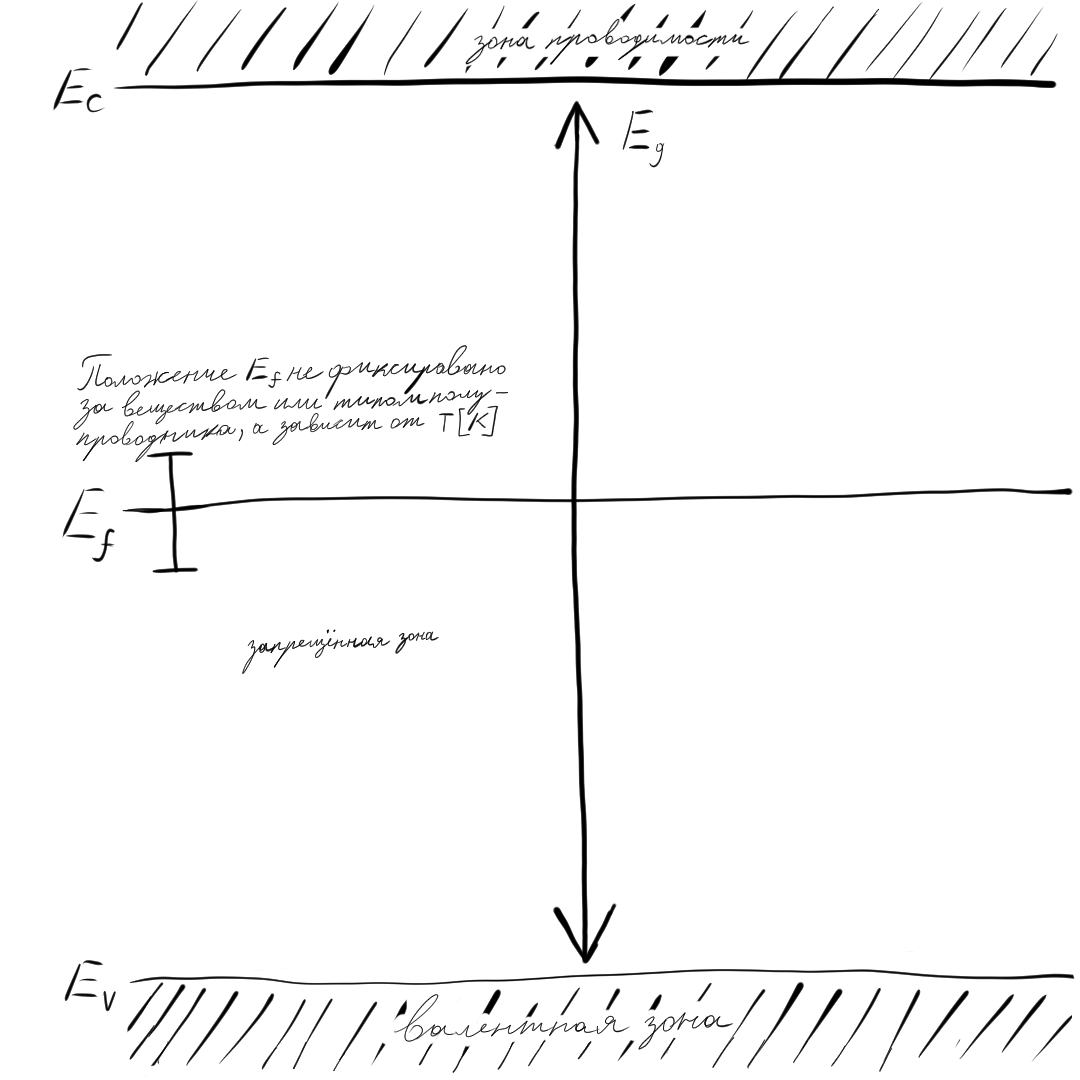
\includegraphics[width=\linewidth]{image/Illustration1.png}
            
            \qquad Функция после подстановки ($\ref{eq:1}$) приводится к 
            \begin{equation*}
                \begin{aligned}
                    f(E) = \frac{1}{\exp{\frac{E-E_f}{kt}} + 1} = 
                    \exp{\left(-\frac{\frac{E_g}{2} - 0.05}{\luaexec{tex.sprint(value_with_mantice(8.617 * 10^(-5) * 300, 5, -2, 0))}}\right)} = 
                    \\
                    = \exp{\left(-\frac{E_g}{\luaexec{tex.sprint(value_with_mantice(2 * 8.617 * 10^(-5) * 300, 5, -2, 0))}} + \luaexec{tex.sprint(value_with_mantice(0.05 / (8.617 * 10^(-5) * 300), 5, 0, 0))}\right)} 
                \end{aligned}
            \end{equation*}
        \end{minipage}
    \end{figure}
    \item Найти концентрацию носителей в \ce{Si} при $T=300$ K.
    
    \section*{solution}

    \quad Возможно нахождение концентрации носителей отрицательного заряда ($n_0$) и 
    положительного заряда ($p_0$) посредством уравнений
    \begin{equation*}
        n_0 = N_c \exp{\left(-\frac{E_c-E_f}{kT}\right)} 
        \hspace{5em} 
        p_0 = N_v \exp{\left(-\frac{E_f-E_v}{kT}\right)}
    \end{equation*}
    в случае поставленной задачи условие приблежения распределения Ферми-Дирака к 
    распределению Максвелла-Больцмана выполняется по умолчанию.

    \quad Эффективные концентрации уровней в свою очередь находятся посредством 
    уравнений
    \begin{equation*}
        N_c = 2 \cdot \left(\frac{2\pi m_c kT}{h^2}\right)^{\frac{3}{2}}
        \hspace{5em}
        N_v = 2 \cdot \left(\frac{2\pi m_v kT}{h^2}\right)^{\frac{3}{2}}
    \end{equation*}

    \begin{figure}[H]
        \hspace{2em}
        \begin{minipage}[t]{0.3\textwidth}
            \vspace{0em}
            \begin{tabularx}{\linewidth}{|X|X|}
                \hline
                Дано \\
                \hline
                $T = 300$ К \\
                $kT = 0.025$ эВ \\
                $N_c = 2.8 \cdot 10^{19}$ см$^{-3}$ \\
                \hline
                Вариант $1$ \\
                \hline
                тип дырок: $n_0$ \\
                $E_c - E_f = 1$ эВ \\
                \hline
                Найти \\
                \hline
                $n_0 - ?$ \\
                \hline
            \end{tabularx}

            \vspace{1em}
            
            \qquad Необходимые данные для численного решения даны, посему 
            подставляем
            \begin{equation*}
                \begin{aligned}
                    n_0 &= 2.8 \cdot 10^{19} \cdot \exp{\left(-\frac{1}{0.025}\right)}
                    \\
                    n_0 &= \luaexec{tex.sprint(value_with_mantice(2.8 * 10^19 * 2.8^(-1/0.025), 5, 1, 0))} \text{ см}^{-3}
                \end{aligned}
            \end{equation*} 

            Ответ: концентрация электронов в кремнии равна $n_0 = \luaexec{tex.sprint(value_with_mantice(2.8 * 10^19 * 2.8^(-1/0.025), 5, 1, 0))} \text{ см}^{-3}$.
        \end{minipage} \hfill
        \begin{minipage}[t]{0.7\textwidth}
            \vspace{0em}
            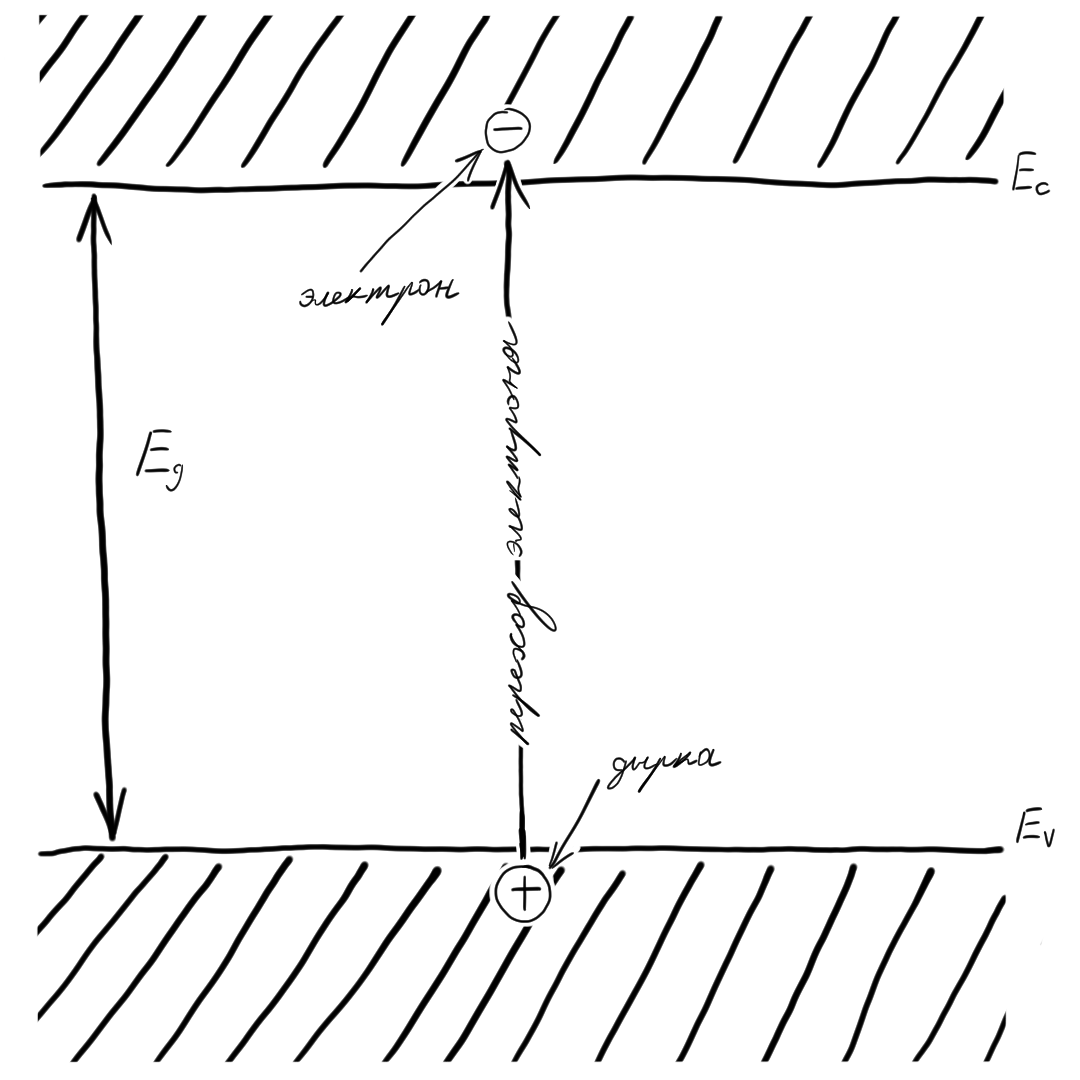
\includegraphics[width=\linewidth]{image/Illustration2.png}
        \end{minipage}
    \end{figure}

    \item Найти концентрацию электронов и дырок в \ce{Si} при $T = 300$ К, при 
    заданных концентрациях донорной и акцепторной примеси. Считать примесь 
    полностью ионизованной.

    \qquad Закон сохранения заряда выполняется на каждом микрообъёме полупроводника
    \begin{equation*}
        {N_a}^- + n_0 = {N_d}^+ + p_0
    \end{equation*}
    также справедлив закон действующих масс, так как распределение электронов и 
    дырок апроксимизируется до статистики Максвелла-Больцмана
    \begin{equation*}
        n_0 \times p_0 = {n_i}^2
    \end{equation*} 

    \begin{figure}[H]
        \hspace{2em}
        \begin{minipage}[t]{0.3\textwidth}
            \vspace{0em}
            \begin{tabularx}{\linewidth}{|X|}
                \hline
                Дано \\
                \hline
                \ce{Si} с ионизованной примесью \\
                $T = 300$ К \\
                $\ce{Si}: n_i = 1.45 \cdot 10^{10}$ см$^{-3}$ \\
                \hline
                Вариант $1$ \\
                \hline
                $N_d = 10^{14}$ см$^{-3}$ \\ 
                $N_a = 0$ \\
                \hline
                Найти \\
                \hline
                $n_0 - ?$ \\
                $p_0 - ?$ \\
                \hline
            \end{tabularx}

            \vspace{1em}

            \qquad Из закона сохранения заряда и условия задачи
            \begin{equation*}
                {N_d}^+ + p_0 - n_0 = 0
            \end{equation*}
            из закона действующих масс 
            \begin{equation*}
                \begin{aligned}
                    {N_d}^+ + \frac{{n_i}^2}{n_0} - n_0 = 0 \\
                    {n_i}^2 + {N_d}^+ n_0 - {n_0}^2 = 0 
                \end{aligned}
            \end{equation*}
            решением будет
            \begin{equation*}
                \begin{aligned}
                    (n_0)_1 = \frac{{N_d}^+ + \sqrt{\left({N_d}^+\right)^2 + 4{n_i}^2}}{2} \\
                    (n_0)_2 = \frac{{N_d}^+ - \sqrt{\left({N_d}^+\right)^2 + 4{n_i}^2}}{2}
                \end{aligned}
            \end{equation*}
            Ответ: концентрация электронов $n_0 = 10^{14}$ и дырок $p_0 = \luaexec{tex.sprint(value_with_mantice(((1.45 * 10^(10))^2)/(10^(14)), 3, 0, 0))}$.
        \end{minipage}
        \begin{minipage}[t]{0.7\textwidth}
            \vspace{0em}
            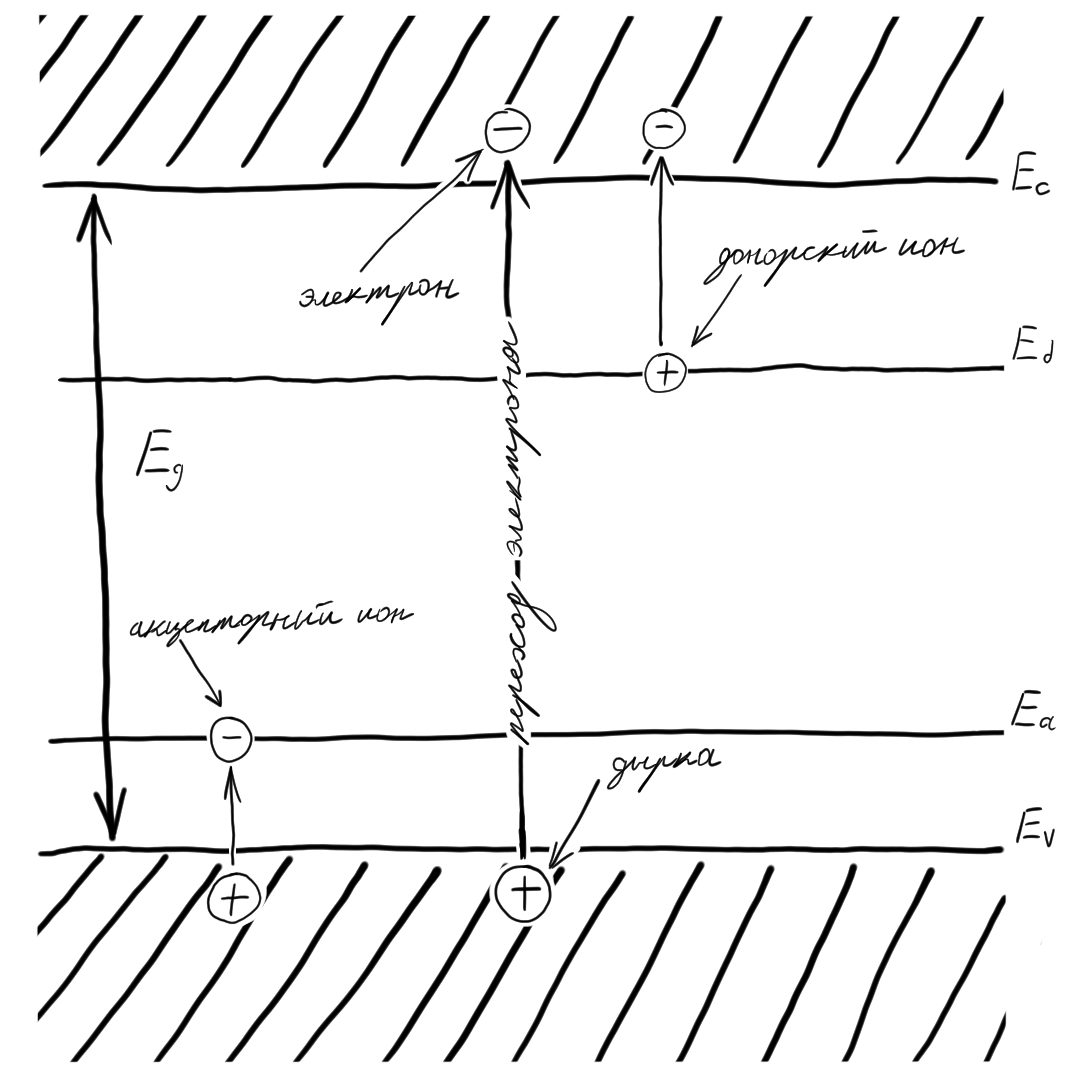
\includegraphics[width=\linewidth]{image/Illustration3.png}
            \vspace{1em}
            \qquad Одно из решений отрицательное, поэтому отсекается
            \begin{equation*}
                \begin{matrix}
                    n_0 = \frac{10^{14} - \sqrt{\left(10^{14}\right)^2 + 4 \cdot 1.45 \cdot 10^{10}}}{2} = \luaexec{tex.sprint(value_with_mantice((10^(14) - ((10^(14))^2 + 4 * 1.45 * 10^(10))^(0.5)) / 2, 5, 0, 0))} & p_0 = \frac{{n_i}^2}{n_0} \\
                    n_0 = \frac{10^{14} + \sqrt{\left(10^{14}\right)^2 + 4 \cdot 1.45 \cdot 10^{10}}}{2} = \luaexec{tex.sprint(value_with_mantice((10^(14) + ((10^(14))^2 + 4 * 1.45 * 10^(10))^(0.5)) / 2, 5, 0, 0))} & p_0 = \frac{\left(1.45 \cdot 10^{10}\right)^2}{10^{14}}=\luaexec{tex.sprint(value_with_mantice(((1.45 * 10^(10))^2)/(10^(14)), 3, 0, 0))}
                \end{matrix}
            \end{equation*}
        \end{minipage}
    \end{figure}

    \item Найти концентрацию электронов и дырок в \ce{Ge} при $Т = 300$ К, при 
    заданных концентрациях донорной и акцепторной примеси. Считать примесь 
    полностью ионизованной.

    \begin{figure}[H]
        \hspace{2em}
        \begin{minipage}[t]{0.3\textwidth}
            \vspace{0em}
            \begin{tabularx}{\linewidth}{|X|}
                \hline
                Дано \\
                \hline
                \ce{Ge} с ионизованной примесью \\
                $T = 300$ К \\
                $\ce{Ge}: n_i = 2.4 \cdot 10^{13}$ см$^{-3}$ \\
                \hline
                Вариант $1$ \\
                \hline
                $N_d = 10^{14}$ см$^{-3}$ \\ 
                $N_a = 0$ \\
                \hline
                Найти \\
                \hline
                $n_0 - ?$ \\
                $p_0 - ?$ \\
                \hline
            \end{tabularx}

            \vspace{1em}

            \qquad Из закона сохранения заряда и условия задачи
            \begin{equation*}
                {N_d}^+ + p_0 - n_0 = 0
            \end{equation*}
            из закона действующих масс 
            \begin{equation*}
                \begin{aligned}
                    {N_d}^+ + \frac{{n_i}^2}{n_0} - n_0 = 0 \\
                    {n_i}^2 + {N_d}^+ n_0 - {n_0}^2 = 0 
                \end{aligned}
            \end{equation*}
            решением будет
            \begin{equation*}
                \begin{aligned}
                    (n_0)_1 = \frac{{N_d}^+ + \sqrt{\left({N_d}^+\right)^2 + 4{n_i}^2}}{2} \\
                    (n_0)_2 = \frac{{N_d}^+ - \sqrt{\left({N_d}^+\right)^2 + 4{n_i}^2}}{2}
                \end{aligned}
            \end{equation*}
            Ответ: концентрация электронов $n_0 = 10^{14}$ и дырок $p_0 = \luaexec{tex.sprint(value_with_mantice(((2.4 * 10^(13))^2)/(10^(14)), 3, 0, 0))}$.
        \end{minipage}
        \begin{minipage}[t]{0.7\textwidth}
            \vspace{0em}
            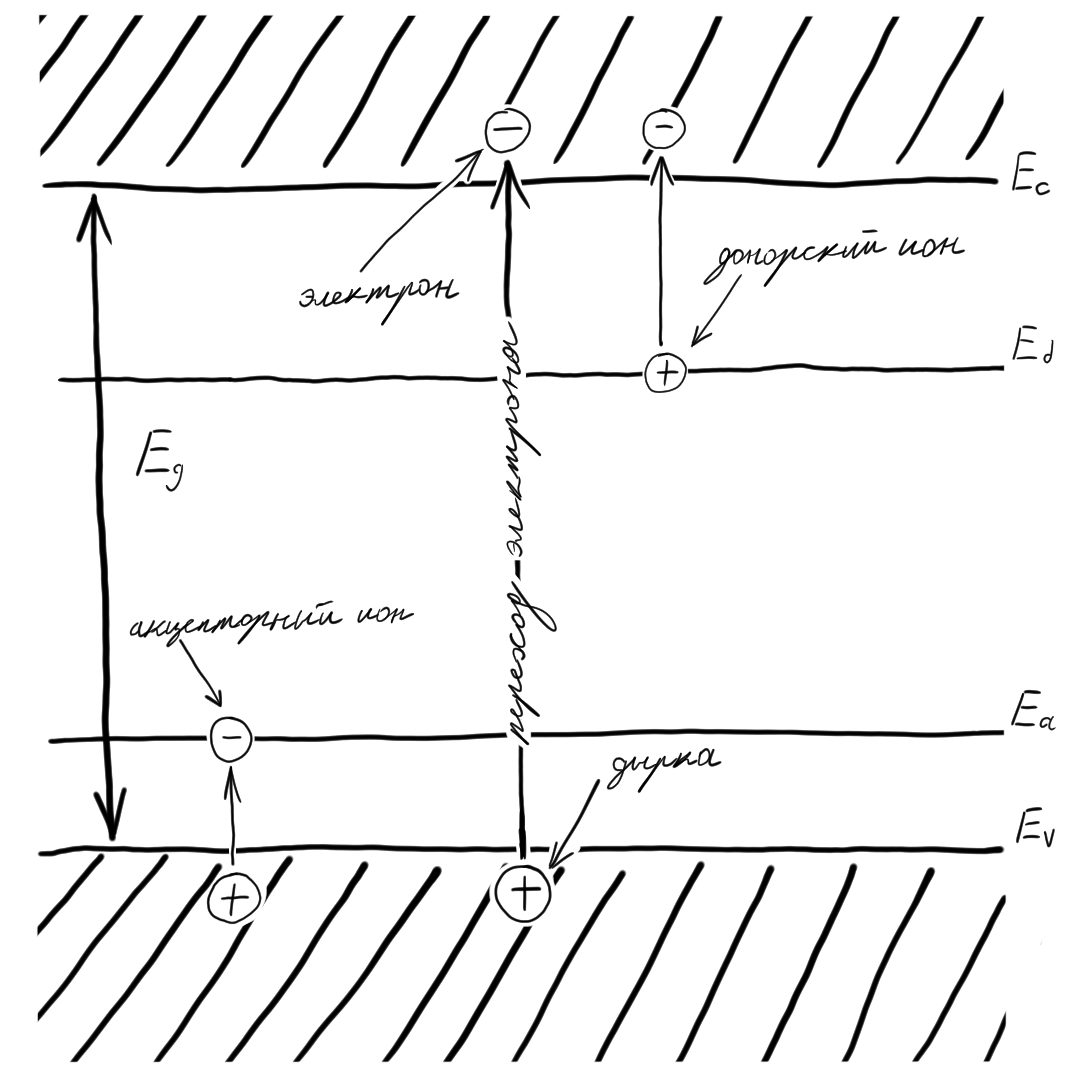
\includegraphics[width=\linewidth]{image/Illustration3.png}
            \vspace{1em}
            \qquad Одно из решений отрицательное, поэтому отсекается
            \begin{equation*}
                \begin{aligned}
                    n_0 = \frac{10^{14} - \sqrt{\left(10^{14}\right)^2 + 4 \cdot 2.4 \cdot 10^{13}}}{2} = \luaexec{tex.sprint(value_with_mantice((10 ^ 14 - ((10 ^ 14) ^ 2 + 4 * 2.4 * 10^(13))^(0.5)) / 2, 5, -1, 0))} \\
                    n_0 = \frac{10^{14} + \sqrt{\left(10^{14}\right)^2 + 4 \cdot 2.4 \cdot 10^{13}}}{2} = \luaexec{tex.sprint(value_with_mantice((10 ^ 14 + ((10 ^ 14) ^ 2 + 4 * 2.4 * 10^(13))^(0.5)) / 2, 5, 0, 0))} 
                \end{aligned}
            \end{equation*}
            концентрация дырок ищется из концентрации электронов
            \begin{equation*}
                p_0 = \frac{{n_i}^2}{n_0} \qquad p_0 = \frac{\left(2.4 \cdot 10^{13}\right)^2}{10^{14}}=\luaexec{tex.sprint(value_with_mantice(((2.4 * 10^(13))^2)/(10^(14)), 3, 0, 0))}
            \end{equation*}
        \end{minipage}
    \end{figure}

    \pagebreak
    
    \item Найти удельное сопротивление ($\rho$) собственного полупроводника при 
    $T = 300$ К. Значения подвижностей $\mu_p$, ($\mu_n / \mu_p$) и собственной 
    концентрации носителей ($n_i$) заданы в соответствии с вариантом.

    \qquad Удельная электропроводность ($\sigma$) — складывается из токов дырочных зарядов и 
    токов электронных зарядов
    \begin{equation*}
        \sigma = en_0\mu_n + ep_0\mu_p
    \end{equation*}
    удельное сопротивление ($\rho$) в свою очередь величина обратная удельной электропроводности ($\sigma$).

    \begin{figure}[h]
        \begin{minipage}[t]{0.28\textwidth}
            \vspace{0em}
            \begin{tabularx}{\linewidth}{|X|}
                \hline
                Дано \\
                \hline
                $T = 300$ К \\
                $e = 1.6 \cdot 10^{-19}$ Кл \\
                \hline
                Вариант $1$ \\
                \hline
                $\mu_n/\mu_p = 1.0$ \\
                $\mu_p = 100 \frac{\text{см}^2}{\text{В} \cdot \text{с}}$ \\
                $n_i = 10^6$ см$^{-3}$ \\
                \hline
                Найти \\
                \hline
                $\rho - ?$ \\
                \hline
            \end{tabularx}

            \vspace{1em}

            \qquad Так как полупроводник нелигированный, то
            \begin{equation*}
                n_0 = p_0 = n_i
            \end{equation*}
            из условия 
            \begin{equation*}
                \mu_n = \mu_p
            \end{equation*}
            из этого формула переписывается как 
            \begin{equation*}
                \begin{aligned}
                    \sigma &= 2en_i\mu_p = \\ 
                    &= 2 \cdot 1.6 \cdot 10^{-19} \cdot 10^6 \cdot 10^2 = \\ 
                    &= \luaexec{tex.sprint(value_with_mantice(2 * 1.6 * 10^(-19) * 10^6 * 10^2, 5, 0, 0))}
                    \\ 
                    \rho &= \frac{1}{\sigma} = \frac{1}{\luaexec{tex.sprint(value_with_mantice(2 * 1.6 * 10^(-19) * 10^6 * 10^2, 5, 0, 0))}} = 
                    \luaexec{tex.sprint(value_with_mantice(1/(2 * 1.6 * 10^(-19) * 10^6 * 10^2), 5, 0, 0))}
                \end{aligned}
            \end{equation*}
            Ответ: удельное сопротивление $\rho = \luaexec{tex.sprint(value_with_mantice(1/(2 * 1.6 * 10^(-19) * 10^6 * 10^2), 5, 0, 0))} \text{ Ом} \cdot \text{см}$.
        \end{minipage} \hfill
        \begin{minipage}[t]{0.68\textwidth}
            \vspace{0em}
            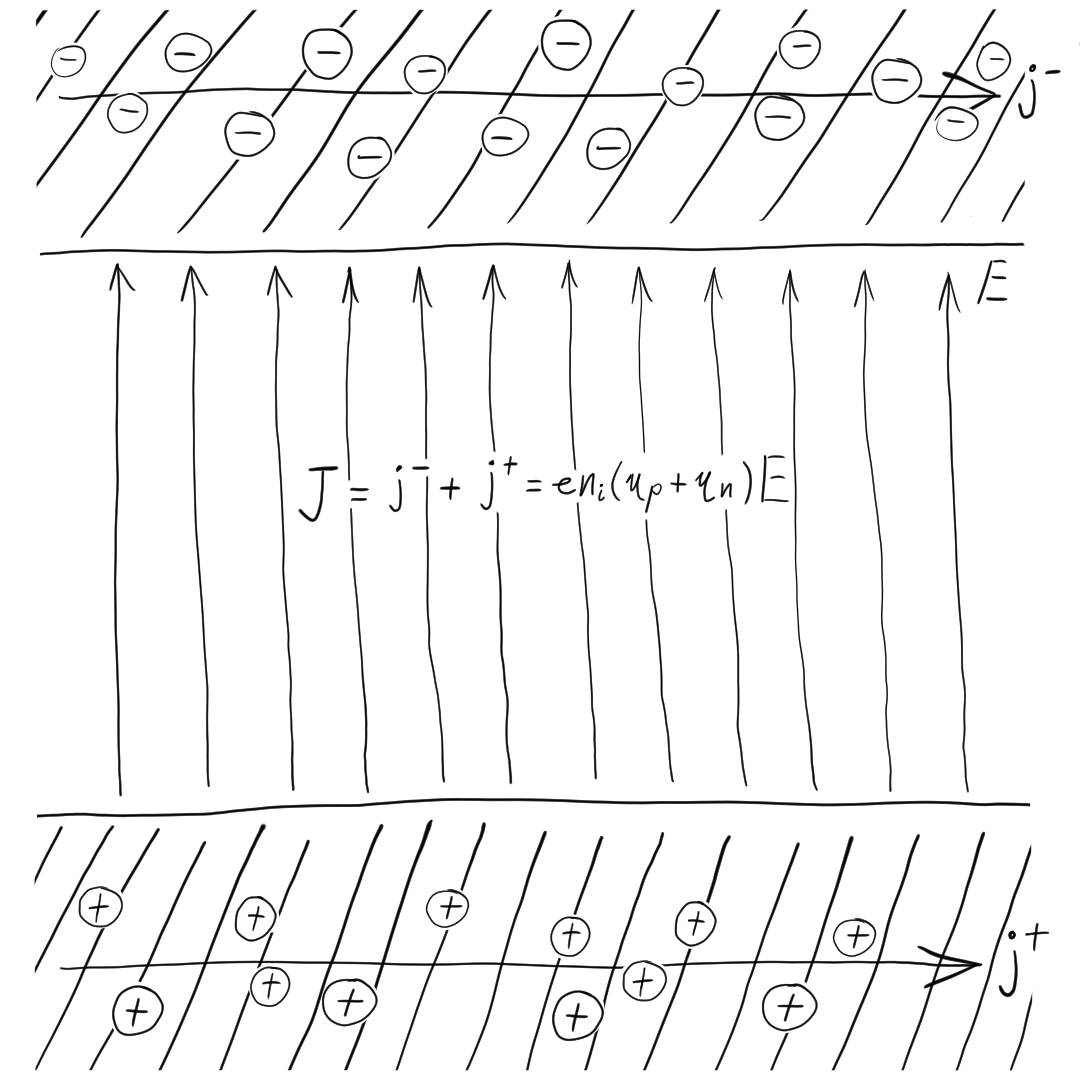
\includegraphics[width=\linewidth]{image/Illustration5.png}
        \end{minipage}
    \end{figure}
\end{enumerate}





\end{document}